\documentclass[10pt,a4paper]{article}

%%%%%%%%%%%%%%%%%%%%%%%%% packages %%%%%%%%%%%%%%%%%%%%%%%%

%\documentclass{aimsessay}
\usepackage[utf8]{inputenc}
\usepackage[english]{babel}

%Import the natbib package and sets a bibliography  and citation styles
\usepackage[round]{natbib}
\usepackage{amsmath}
\usepackage{amssymb}
%\usepackage{natbib}
\usepackage{amsthm}
\usepackage{amsfonts}
\usepackage{graphicx}
%\usepackage{siunitx}
%\usepackage[utf8]{inputenc}
%\usepackage[english]{babel}
\usepackage[all]{xy}
\usepackage{float}
\usepackage{tikz}
\usepackage{verbatim}
\usepackage[left=2cm,right=2cm,top=2.3cm,bottom=2.5cm]{geometry}
\usepackage[hidelinks]{hyperref}
\hypersetup{
	colorlinks=false,
	linkcolor=blue,
	filecolor=magenta,      
	urlcolor=cyan,
	pdftitle={Overleaf Example},
	pdfpagemode=FullScreen,
}
\usepackage{caption}
\usepackage{subcaption}
\usepackage{psfrag}

\usepackage{url} 
%\bibliographystyle{abbrvnat}
\usepackage{booktabs}  
\usepackage[T1]{fontenc}    % use 8-bit T1 fonts
%\usepackage[nottoc]{tocbibind}

\usepackage{url} 

\newcommand{\donna}[1]{{\color{red}{#1}}}   
\newcommand{\ignore}[1]{}

%%%%%%%%%%%%%%%%%%%%% students data %%%%%%%%%%%%%%%%%%%%%%%%
\newcommand{\student}{Brian KYANJO }
\newcommand{\course}{Prof. Jodi Mead, Michal Kopera, and Dylan Mikesell}
\newcommand{\assignment}{ Prof. Donna Calhoun}


%%%%%%%%%%%%%%  Shortcut for usual set of numbers  %%%%%%%%%%%

\newcommand{\N}{\mathbb{N}}
\newcommand{\Z}{\mathbb{Z}}
\newcommand{\Q}{\mathbb{Q}}
\newcommand{\R}{\mathbb{R}}
\newcommand{\C}{\mathbb{C}}

%%%%%%%%%%%%%%%%%%%%%%%%%%%%%%%%%%%%%%%%%%%%%%%%%%%%%%%555
\begin{document}
	
	%%%%%%%%%%%%%%%%%%%%%%% title page %%%%%%%%%%%%%%%%%%%%%%%%%%
	\thispagestyle{empty}
	\begin{center}
		\textbf{A Riemann Solver for Wet/Dry Interfaces in Finite Volume Schemes\\[0.5cm]
			Synthesis Paper}
		\vspace{.2cm}
	\end{center}
	
	%%%%%%%%%%%%%%%%%%%%% assignment information %%%%%%%%%%%%%%%%
	
	\begin{center}
		\rule{17cm}{0.2cm}\\[0.3cm]
	\end{center}	
	
	\noindent	Name: \student \hfill Supervisor: \assignment\\[0.1cm]
	Committee: \course \hfill Date: \today\\
	\rule{17cm}{0.05cm}
	\vspace{.2cm}
	
	\section{Introduction}
	
				A tsunami is a series of energetic water waves generated due to the displacement of large volumes of water by different mechanisms such as earthquakes, volcanic eruptions, underwater landslides, and local landslides along the coast. According to the recent tragic events in December 2004 in Indonesia and  South Africa, tsunamis may be extremely catastrophic: they can lead to the loss of human lives and destroy buildings and roads. Typically, they cause devastative damages to infrastructures. Deep knowledge of tsunamis is required to provide early warning messages to the regions that may be affected, carry out necessary evacuations, and also anticipate the highest run-ups and run-downs    (\cite{sanchez2016uncertainty,dutykh2007water,dias2007dynamics}).
				
				Most numerical tsunami models rely on solving Riemann problems which can robustly track wetting and drying interfaces to model run-up on beaches and inundation into harbors and communities along the affected coastlines.  Various approaches have been taken to handle these wetting and drying states. For instance, \citet{ge:2011,li-ta-wa-ca-ba-ch-li:2021,fivser2016mass} used Godunov-type finite volume methods to model inundation by allowing cells to shift from dry to wet near refinement boundaries dynamically. Furthermore, \citet{barzgaran2019numerical}  used an augumented Riemann solver coupled with a second-order finite volume method to simulate bedload sediment transport. Results proved that this efficient method is capable of modeling wet/dry interfaces and investigated flow regimes. In addition, the technique employed wave decomposition and the flux-wave formula, which made bed variations vary as four waves propagated from each cell interface. Many more other techniques to manage dry/wet interfaces have been proposed by various researchers in unique ways, for instance, see \citet{po:2015, po:2018, pe-bo-ma:2011, toro2001shock, chaabelasri1849simple,nikolos2009unstructured,huang2013well, bi2014finite,song2011unstructured,buttinger2019fast}.
		

	\section{Shallow water equations for tsunami modeling}
	\label{sec2}
	Shallow water models have been frequently used to handle the propagation of tsunami waves in the ocean see for instance \citet{dutykh2007water,le-ge-be:2011,dias2007dynamics}. The SWE assumption is applicable as the average ocean depth is very shallow compared to the tsunami's wavelength. In addition, the amplitude of tsunami is minimal offshore, typically less than 1m, to justify the shallowness assumption. 
	
		The shallow water wave equations (SWE) are a system of hyperbolic partial differential equations (PDEs) governing the flow below a pressure surface in a fluid. They arise from the Navier-Stokes equations.  In one dimension, the SWE  can be used to model a fluid in a channel of unit width, taking the vertical velocity negligible and horizontal velocity roughly constant throughout any cross-section of the channel (\cite{ge:2008}).  
		
		Consider small-amplitude waves in a one-dimensional fluid channel that is shallow relative to its wavelength. The conservation mass and of momentum equation is written in terms of height $h(t)$, momentrum $hu$ and  pressure, $p(x,t) = \frac{1}{2}\rho gh^{2}$, which breaks down into system \eqref{p2}
	\begin{equation}
		\begin{aligned}
			h_{t} + (hu)_x &= 0 \\
			(hu)_t + \left(hu^{2} + \frac{1}{2}\rho gh^{2} \right)_x & = 0 
		\end{aligned}
		\label{p2}
	\end{equation}	
	where $hu$ measures the flow rate of water past a point,  $\rho$ $(kg/m^{3})$ is the constant density of the in-compressible fluid, and $u(x,t)$ ($m/s$) is the horizontal velocity  (\cite{leveque2002finite,toro2001shock}).  We will set $\rho = 1$ here.
	
	A simple set of initial conditions is a single discontinuity at the middle of the channel.  In this case, we set $h$ and $hu$ equal to constants on either side of the medium.  This problem is a classic Riemann Problem, and the SWE has an exact solution.  We assume the discontinuity is at $x = 0$; its associated Riemann problem is the initial value problem initial conditions of:
		\begin{eqnarray}
		q(x,0)& =& \begin{cases}
			q_{l}, & \text{if \, $x \le 0,$}\\
			q_{r},& \text{if \, $x > 0,$}\\
			
		\end{cases}  
		\label{rp1}     
	\end{eqnarray}
where $q_{l}$ and $q_{r}$ are two piece-wise constant states separated by a discontinuity. 

	The variation of $h$ and $hu$ on either side of the discontinuity leads the waves in the Riemann problem to move at different speeds creating discontinuities (shocks) or changing regions (rarefactions) (\cite{leveque2002finite}).  At $x = 0$ and $t = 0$,   the discontinuity is located between the left and right state, so the solution at the left ($q_{l}$) and right($q_{r}$) states are given by: 
	\begin{equation}
		q_{l} = \begin{bmatrix}
			h_{l} \\( hu)_{l}
		\end{bmatrix}  \quad \text{and} \quad q_{r} = \begin{bmatrix}
			h_{r} \\( hu)_{r}
		\end{bmatrix} 
		\label{ic}
	\end{equation}
	As $t$ increases, four distinct regions are created, separated by characteristics. The middle state called the intermediate state($q_{m}$) is generated.  The determination of this state characterizes the Riemann problem and how it connects to other states via waves in each respective characteristic family.  The selection of rarefaction or shock is based on the well-known Lax entropy condition.   For the SWEs, this condition reduces to $h_m > h_l$ for a left going shock; otherwise, a left going rarefaction and $h_m>h_r$ for a right going shock otherwise a right going rarefaction.    Figure \ref{fig:x-tplane} shows a wave combination of a centered rarefaction and shock wave from the first and second characteristic family, respectively.
	
	\begin{figure}[H]
		\centering
		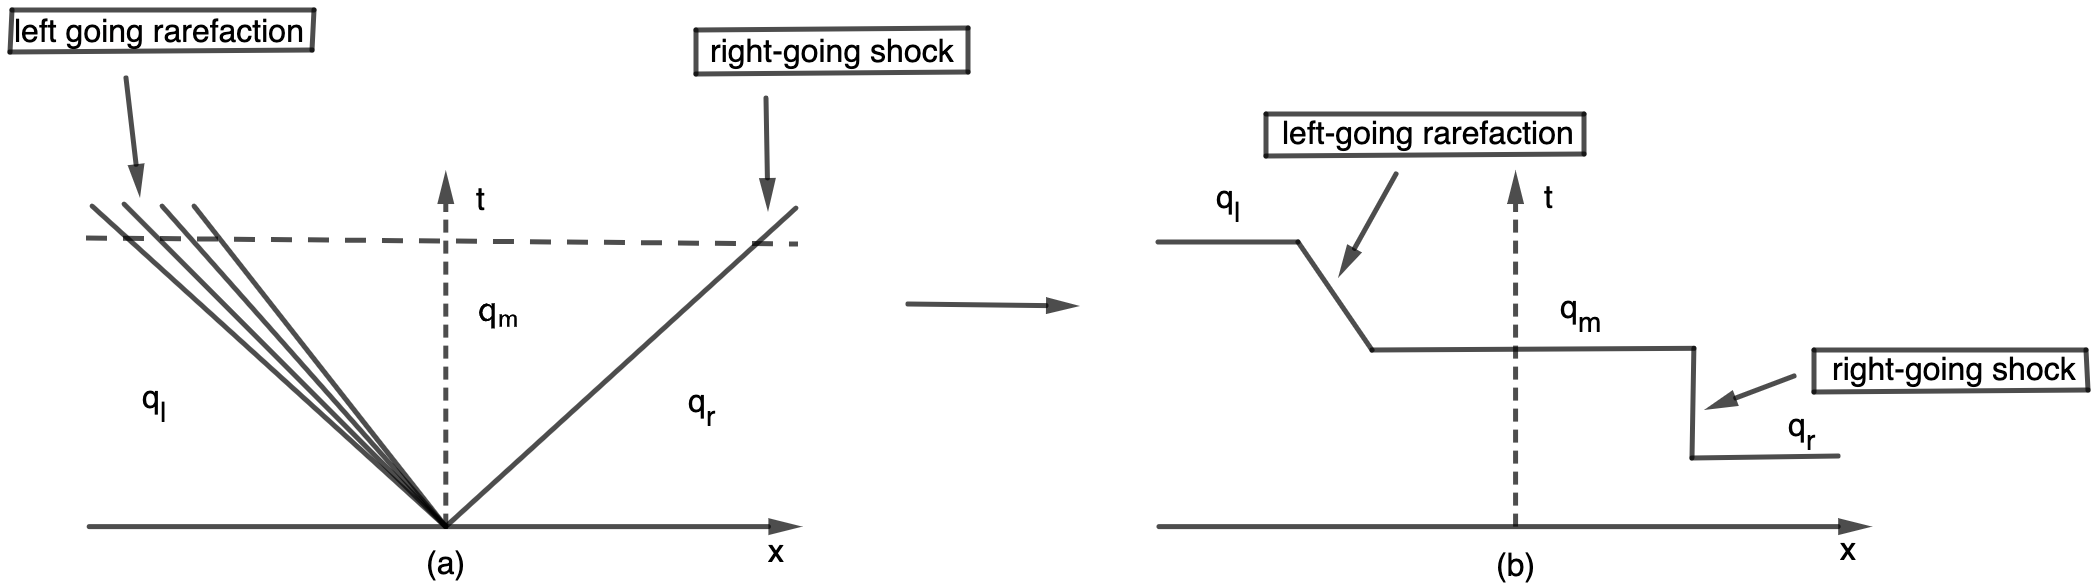
\includegraphics[width=.77\linewidth]{images/geo11}
		\caption{ x-t plane showing the connection of states, {\em left-going rarefaction}, and the {\em right-going shock} are depicted by: (a). Structure of the characteristic curves for the  Riemann solution profile and (b). Actual representation of the states in the Riemann solution.}
		\label{fig:x-tplane}
	\end{figure}
	The intermediate state is obtained by solving the Riemann problem using the exact or approximate method. Approximate methods are widely used due to their cheap computational cost compared to the exact solvers (\cite{roe1981approximate}).
	
	
	Figure \ref{hor2} represents four plots showing initial conditions \ref{fig:t0}, and the temporal evolution of a left going  rarefaction and a right going shock. This solutions are produced by the exact Riemann solver after applying $h_l = 2$, $h_r = 1$, and $u_l = u_r = 0$ as initial conditions in  the Riemann problem.
	
	\begin{figure}[H]
		\subfloat[]{
			\begin{minipage}[c][1\width]{
					0.32\textwidth}
				\centering
				%\caption{}
				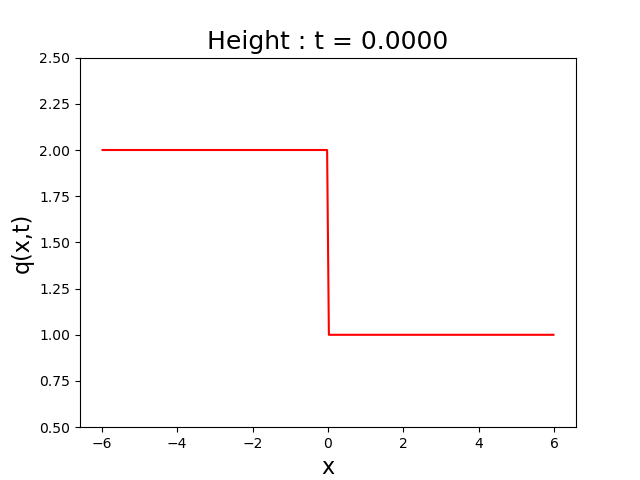
\includegraphics[width=\linewidth, height=5cm]{images/t0}
				\label{fig:t0}
		\end{minipage}}
		\subfloat[]{
			\begin{minipage}[c][1\width]{
					0.32\textwidth}
				\centering
				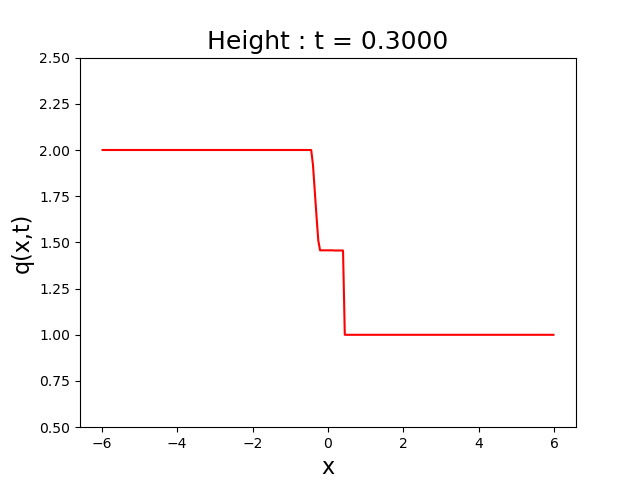
\includegraphics[width=\linewidth, height=5cm]{images/t3}
				\label{fig:t3}
		\end{minipage}}
		\hfill
		\subfloat[]{
			\begin{minipage}[c][1\width]{
					0.32\textwidth}
				\centering
				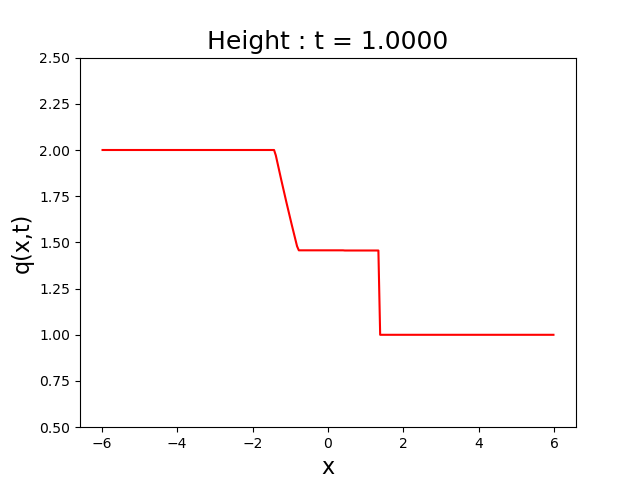
\includegraphics[width=\linewidth,height=5cm]{images/t1}
				\label{fig:t1}
		\end{minipage}}
			\caption{Temporal evolution of the height field solution for the dam break problem with {\em left-going rarefaction} and a {\em right-going shock}  are depicted by (a), (b) and (c) at time steps: $t=0~s$ (initial conditions), $t = 0.3~s$, and $t = 1.0~s$ respectively.  }
		\label{hor2}
	\end{figure}
	
	

	\subsection{Exact Riemann Solver for two-shock SWE}
The states in \ref{fig:x-tplane} are separated by either {\em shocks} or {\em rarefactions}. General left, and right states will be connected by a combination of the two (either two shocks, two rarefactions, or one of each).  We describe how to determine if a shock connects two states.  We refer the reader to \citet{leveque2002finite} for other cases. 

We can achieve an exact solution to the Riemann Problem for the SWE as follows. 
The shock speed, $s(t)$,  from the shock wave as the solution emerges is determined from the Rankine-Hugoniot jump condition given by equation \eqref{e1}  which must be satisfied across any shock wave.  If $q_l$ and $q_r$ are connected by a shock, the Rankine Hugoniot conditions will be satisfied (\cite{leveque2002finite,toro2001shock}).
	\begin{equation}
		\begin{aligned}
			s_1(q_{m} - q_{l}) & = f(q_{m}) - f(q_{l}) \\
			s_2(q_{r} - q_{m}) & = f(q_{r}) - f(q_{m})
		\end{aligned}
		\label{e1}
	\end{equation}
where $f$ is the numerical flux function. \\

By applying condition  \eqref{e1} to shallow water equations \eqref{p2}  creates a system of four equations that must be satisfied simultaneously. The temporal evolution of the height and velocity fields solution at time steps: $t=0~s$ (initial conditions), $t = 0.3~s$, and $t = 1.0~s$ are  depicted in figure \ref{fig:allshock}. The figures: \ref{fig:allshock0}, \ref{fig:allshock3}, \ref{fig:allshock1} in the first row exhibit the evolution of the hight field solution profile from the intial condition to the exact Riemann solution at time $t = 1.0~s$. Similarly figures: \ref{fig:allshockv0}, \ref{fig:allshockv3}, \ref{fig:allshockv1} in the second row show the evolution of the velocity field solution profile from the intial condition to the exact Riemann solution at time $t = 1.0~s$. This solutions are produced by the exact Riemann solver after applying $h_l = h_r = 1$, $u_l  =  0.5$, and $u_r = -0.5$ as initial conditions in  the Riemann problem.
	
	\begin{figure}[htb]
		\centering % <-- added
		\begin{subfigure}{0.33\textwidth}
			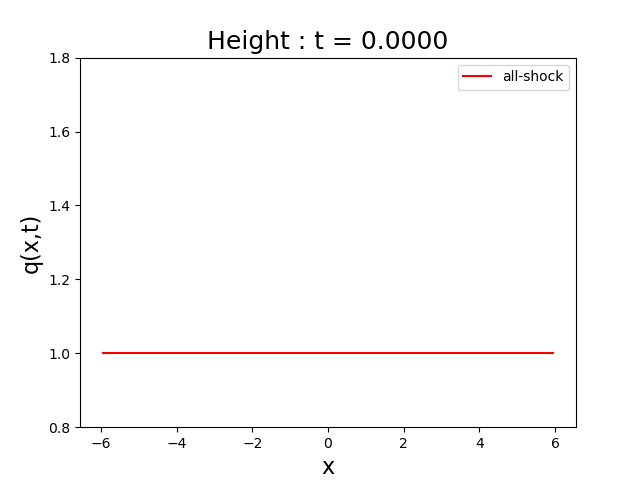
\includegraphics[width=\linewidth]{images/allshock0}
			\caption{  }
			\label{fig:allshock0}
		\end{subfigure}\hfil % <-- added
		\begin{subfigure}{0.33\textwidth}
			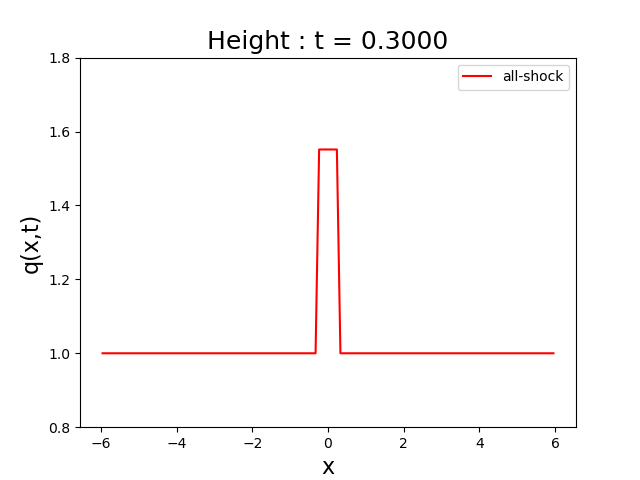
\includegraphics[width=\linewidth]{images/allshock3}
			\caption{}
			\label{fig:allshock3}
		\end{subfigure}\hfil % <-- added
		\begin{subfigure}{0.33\textwidth}
			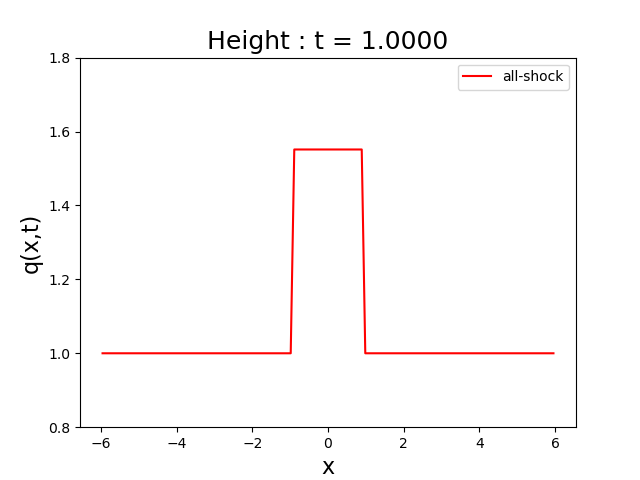
\includegraphics[width=\linewidth]{images/allshock1}
			\caption{}
			\label{fig:allshock1}
		\end{subfigure}
		
		\medskip
		\begin{subfigure}{0.33\textwidth}
			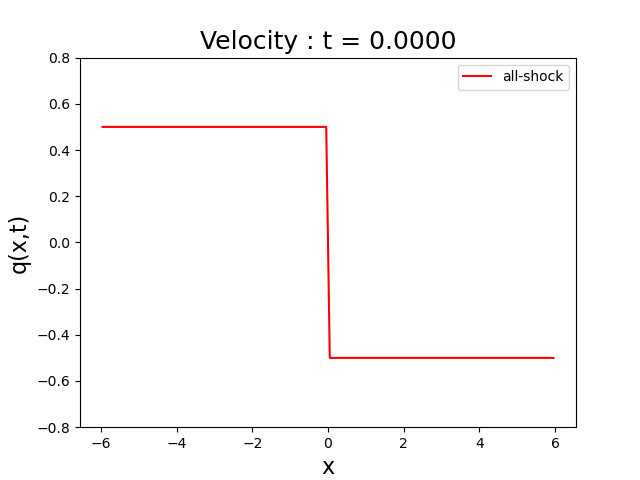
\includegraphics[width=\linewidth]{images/allshockv0}
			\caption{}
			\label{fig:allshockv0}
		\end{subfigure}\hfil % <-- added
		\begin{subfigure}{0.33\textwidth}
			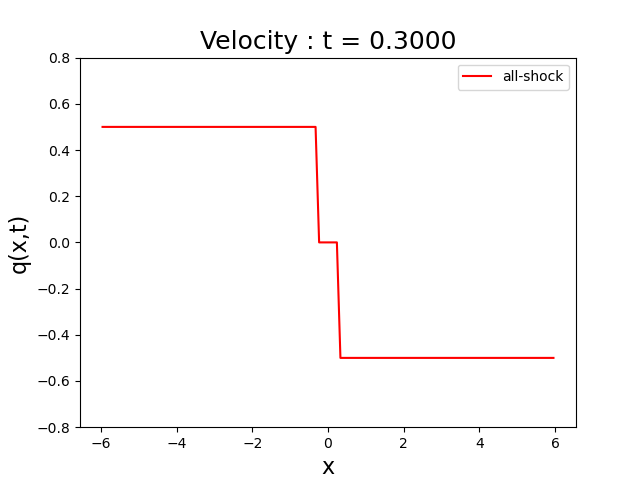
\includegraphics[width=\linewidth]{images/allshockv3}
			\caption{}
			\label{fig:allshockv3}
		\end{subfigure}\hfil % <-- added
		\begin{subfigure}{0.33\textwidth}
			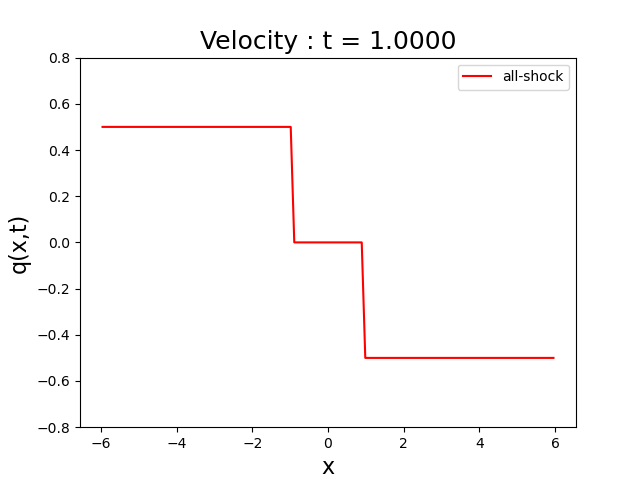
\includegraphics[width=\linewidth]{images/allshockv1}
			\caption{}
			\label{fig:allshockv1}
		\end{subfigure}
		\caption{Temporal evolution of the height and velocity field solution for the all-shock case with {\em left-going shock} and a {\em right-going shock}  are depicted by (a), (b), (c), (d), (e), and (f) at time steps: $t=0~s$ (initial conditions), $t = 0.3~s$, and $t = 1.0~s$. }
		\label{fig:allshock}
	\end{figure}

	\subsection{General case}
The Lax entropy condition requiring that $h_m > h_l, h_r$ may not be satisfied in all cases.  We can also connect states by a rarefaction wave. See Figure (\ref{allrare})  for illustration of the evolution of a Riemann problem  for a case in which both the left and  the right states are connected to the intemediate state by a left going rarefaction and a right going rarefaction wave  respectively.   We refer the reader to \citet{leveque2002finite} for more information about rarefactions.  Figure \ref{fig:allrare0} depicts the intial condition (Riemann problem) solution at  $t=0~s$  and figures \ref{fig:allrare3} and \ref{fig:allrare1} represents the evolution of the height field solution at $t = 0.3~s$, and $t = 1.0~s$.  This solutions are produced by the exact Riemann solver after applying $h_l = h_r = 1$, $u_l  =  -0.5$, and $u_r = 0.5$ as initial conditions in  the Riemann problem.


 

\begin{figure}[H]
	\subfloat[]{
		\begin{minipage}[c][1\width]{
				0.32\textwidth}
			\centering
			%\caption{}
			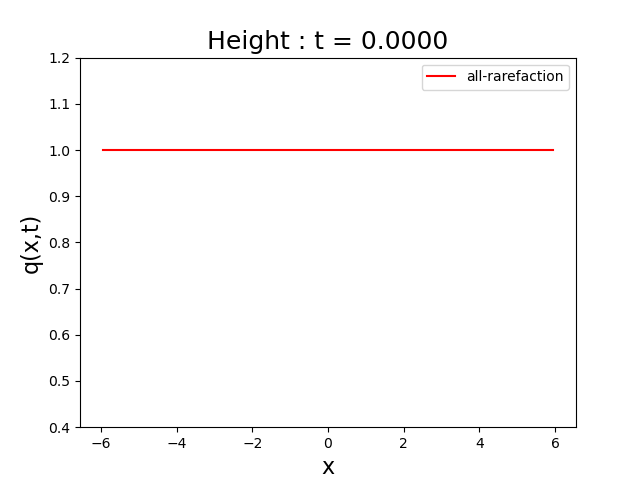
\includegraphics[width=\linewidth, height=5cm]{images/allrare0}
			\label{fig:allrare0}
	\end{minipage}}
	\subfloat[]{
		\begin{minipage}[c][1\width]{
				0.32\textwidth}
			\centering
			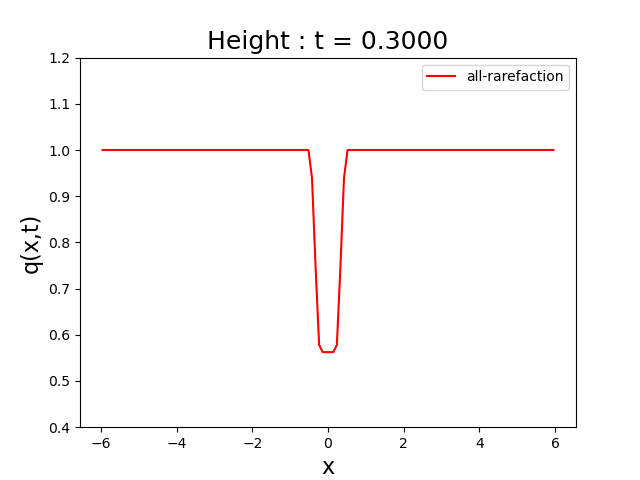
\includegraphics[width=\linewidth, height=5cm]{images/allrare3}
			\label{fig:allrare3}
	\end{minipage}}
	\hfill
	\subfloat[]{
		\begin{minipage}[c][1\width]{
				0.32\textwidth}
			\centering
			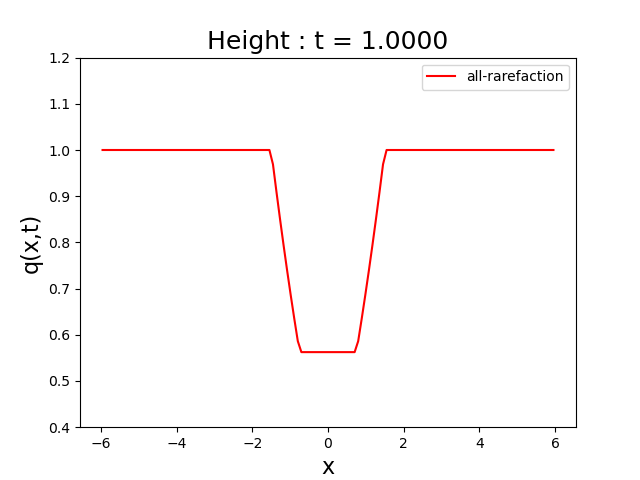
\includegraphics[width=\linewidth,height=5cm]{images/allrare1}
			\label{fig:allrare1}
	\end{minipage}}
	\caption{Temporal evolution of the height field solution for the all-rarefaction case with {\em left-going rarefaction} and a {\em right-going rarefaction}  are depicted by (a), (b) and (c) at time steps: $t=0~s$ (initial conditions), $t = 0.3~s$, and $t = 1.0~s$ respectively.  }
	\label{allrare}
\end{figure}

	\subsection{Finite volume discretization}
Finite volume discretizations are widely used in tsunami modeling since they are: well suited for inundation regimes, robust in the presence of drying regions, well-balanced, and can capture the inundating shoreline and run-up features, see for instance \citet{ge:2008,ge:2011,george2006finite,be-ge-le-ma:2011,bi2014finite,leveque2002finite,ba-le-mi-ro:2003}. The finite volume schemes rely on exact or approximate solutions to the Riemann problem described above.  

Consider a one dimensional (1D) conservation law  (equation \eqref{fvm0}),  where $q$ is the measure of conserved quantity density and $f(q)$ is a flux function

	\begin{equation}
		q_{t}(x,t) + f(q(x,t))_{x} = 0.
		\label{fvm0}
	\end{equation}	
	In finite volume methods (FVM), the domain is broken down into grid cells. Consider $C_{i} = (x_{i-\frac{1}{2}},x_{i+\frac{1}{2}})$ to be the $i^{th}$ grid cell, the average value over the $i^{th}$ interval at time $t^{n}$ is numerically approximated by $Q_{i}^{n}$ in equation \eqref{wpa0}.
	
	\begin{equation}
		Q_{i}^{n} \approx \dfrac{1}{\Delta x} \int_{C_{i}}q(x,t^{n})dx
		\label{wpa0}
	\end{equation}
	where $\Delta t = (t^{n+1} - t^{n})$ and  $\Delta x = (x_{i+\frac{1}{2}} - x_{i-\frac{1}{2}})$ is the cell length. A discontinuity in $q$ violates the PDE in the classical sense and only holds for the integral conservation law (fundamental equation \eqref{fvm1}) \ignore{\cite{leveque2002finite}}. Therefore at grid points near discontinuities where PDEs don't hold, all classical finite difference methods breakdown, resorting to FVM which are based on equation \eqref{fvm1}. 	
	\begin{equation}
		\frac{d}{dt} \int_{c_{i}} q(x,t)dx = f(q(x_{i-\frac{1}{2}},t)) -  f(q(x_{i+\frac{1}{2}},t))
		\label{fvm1}
	\end{equation}	
	The approximate  total integral of $q$ over each grid cell is evaluated and updated at every time step by the grid cell edge fluxes. The determined numerical flux functions evaluate the  cell averages over a certain volume, which are used to approximate the solutions within the cells, using equation \eqref{cellupdate} \ignore{\cite{le-ge-be:2011}}.
	
	\begin{equation}
		Q_{i}^{n+1} = Q_{i}^{n} - \frac{\Delta t}{\Delta x} (F_{i+\frac{1}{2}}^{n} - F_{i-\frac{1}{2}}^{n})
		\label{cellupdate}
	\end{equation}	
	where $F_{i+\frac{1}{2}}^{n} $ is the average flux approximation along $x=x_{i-\frac{1}{2}}$.
	The Riemann problem is a fundamental tool in the evolution of FVM. Taking two neighbouring grid cells: $Q_{i-1} = q_{L}$ and $Q_{i} = q_{R}$ to be cell averages, this information is used by a Riemann solver to compute numerical fluxes ( $F_{i-\frac{1}{2}}^{n} = \mathcal{F}(Q_{i-1} , Q_{i} )$); this returns the middle state.  The flux $f(q)$ is then evaluated at this middle state, that is used to update the cell average at each time step. Then equation \eqref{cellupdate} becomes:
	
	\begin{equation}
		Q_{i}^{n+1} = Q_{i}^{n} - \frac{\Delta t}{\Delta x} \left[ \mathcal{F}(Q_{i} , Q_{i+1} ) - \mathcal{F}(Q_{i-1} , Q_{i} ) \right]
		\label{cellupdat}
	\end{equation}
	where $\mathcal{F}$ is the  numerical flux function $F_{i-\frac{1}{2}}^{n}$ at $q_l = Q_{i-1}$  and $q_r = Q_{i}$.
	
The above  scheme is essentially the original Godunov scheme \cite{godunov1959difference} and is only first order accurate.  Different finite volume schemes will include higher order time stepping and or spatial terms to increase accuracy.  For instance, figures \ref{fig:exap} and \ref{fig:exapp}, depicts the first and second-order finite volume solutions and compares them to the true solution described in Section \ref{sec2} for the dam break problem height field simulated at the final time with limiters. Figure \ref{fig:exap}  shows that the first-order approximate solution does not coincide with the exact solution at region edges. However, the second order approximate solution \ref{fig:exapp}  fits the exact solution accurately; hence this validates the exact and numerical solutions.
	\begin{figure}[H]
		\begin{subfigure}[b]{0.5\textwidth}
			\centering
			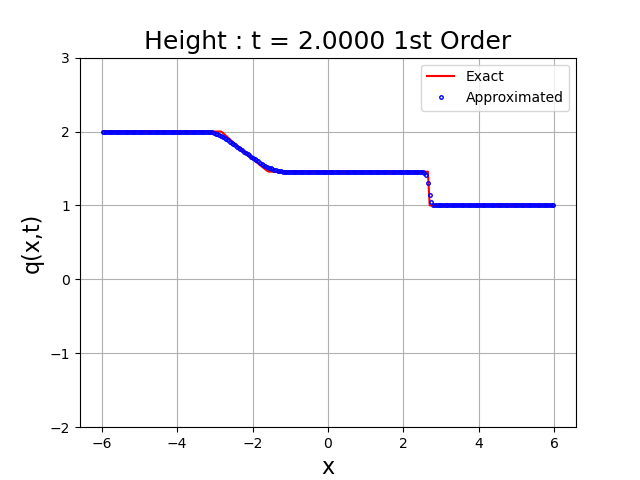
\includegraphics[width=1.0\linewidth]{images/exap}
			\caption{}
			\label{fig:exap}
		\end{subfigure}
		%
		\begin{subfigure}[b]{0.5\textwidth}
			\centering
			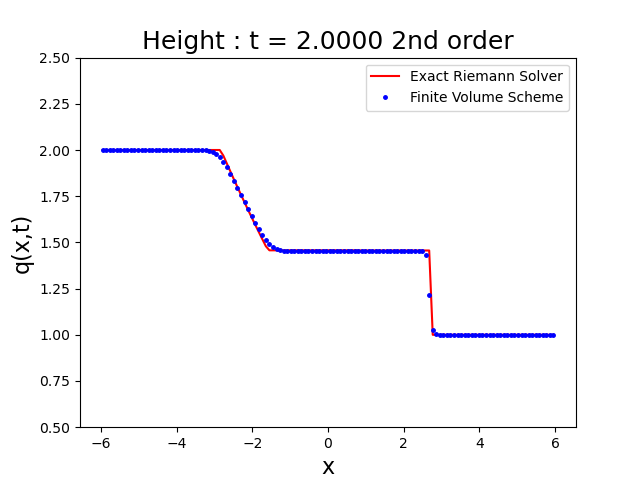
\includegraphics[width=1.0\linewidth]{images/exapp}
			\caption{}
			\label{fig:exapp}
		\end{subfigure}
		\caption{(a) and (b) respectively show height field at the final time step for both first and second order correction with limiters for the exact and approximate solutions.}
	\end{figure}


	\subsection{Finite schemes in quasi-linear form}
	Another approach to solving conservation laws is to write  them in  {\em quasilinear form} and develop numerical methods based on an eigen-decomposition of the Jacobian matrix. The general conservation law in equation\eqref{fvm0} can be written in {\em quasi-linear form}
as
\begin{equation}
	q_{t} + f'(q)q_{x} = 0
	\label{wpa3}
\end{equation}
where  $f'(q) \in \mathbb{R}^{m\times m}$  flux Jacobian matrix.  Consider a Riemann problem for the system  \eqref{wpa3} with initial data 

\begin{equation}
	q(x,t^n)  = \begin{cases}
		Q_{i-1}^{n}  & \text{if} \quad  x < x_{i-\frac{1}{2}}\\
		Q_{i}^{n} & \text{if} \quad x > x_{i-\frac{1}{2}}\\
	\end{cases}    
	\label{w4}   
\end{equation}
\subsubsection{Wave Propagation algorithm (WPA)}
 Here the formalism of the WPA, first described in \cite{le:1997} is presented.   The initial data (equation \eqref{w4}), is used by the exact Riemann solver to generate an intermediate state ($q_m = (h_m, hu_m)^T$), which is used to evaluate the eigenvalues ($\lambda_{i-1/2}$) and eigenvectors ($r_{i-1/2}$) at $x = x_{i-\frac{1}{2}}$. The $p^{th}$ wave at interface $i-1/2$ is given by $\mathcal W^p_{i-1/2} \equiv \alpha_{i-\frac{1}{2}} r^p_{i-\frac{1}{2}}$ with speeds $s^p_{i-1/2} = \lambda^p_{i-1/2}$, where $ \alpha_{i-\frac{1}{2}}$ depicts the coefficients of the the eigenvectors.  Waves and speeds are obtained as an eigenvector decomposition of the jump in $Q_i$ at the interface $i-\frac{1}{2}$.  This decomposition takes the form

\begin{equation}
	Q_{i} -  Q_{i-1} = \sum_{p=1}^{m}  \alpha_{i-\frac{1}{2}} r_{i-\frac{1}{2}} \equiv \sum_{p=1}^{m} \mathcal{W}_{i-\frac{1}{2}}^{p}
	\label{wpa19}
\end{equation}
The wave speed $s_{i-\frac{1}{2}}^{p}$ associated with the vector $r_{i-\frac{1}{2}}^{p}$, are preselected basing on the characteristic structure of the initial Riemann data. Therefore the fluctuations $\mathcal{A^{+}}\Delta Q_{i-\frac{1}{2}}^{n}$  and $\mathcal{A^{-}}\Delta Q_{i-\frac{1}{2}}^{n} $ are defined by equations \eqref{f0} and \eqref{f1}:

\begin{eqnarray}
	\mathcal{A^{-}}\Delta Q_{i-\frac{1}{2}}^{n} = \sum_{\{ p:s_{i-\frac{1}{2}}^{p}<0\}} s_{i-\frac{1}{2}}^{p} \mathcal{W}_{i-\frac{1}{2}}^{p}
	\label{f0}\\
	\mathcal{A^{+}}\Delta Q_{i-\frac{1}{2}}^{n} =\sum_{\{ p:s_{i-\frac{1}{2}}^{p}>0\}} s_{i-\frac{1}{2}}^{p} \mathcal{W}_{i-\frac{1}{2}}^{p}
	\label{f1}
\end{eqnarray}

	The second order accuracy is obtained by taking the correction terms into account as shown described in equation \eqref{wpa2} 

\begin{equation}
	Q_{i}^{n+1} =  Q_{i}^{n} - \frac{\Delta t}{\Delta x}(\mathcal{A^{+}}\Delta 	Q_{i-\frac{1}{2}}^{n} + \mathcal{A^{-}}Q_{i+\frac{1}{2}}^{n}) -  \frac{\Delta t}{\Delta x} (\tilde{F}_{i+\frac{1}{2}}^{n} - \tilde{F}_{i-\frac{1}{2}}^{n} )
	\label{wpa2}
\end{equation}
where $\tilde{F}_{i-\frac{1}{2}}^{n} $ are second order correction terms determined by the waves and speeds in the Riemann problems after approximating the average flux along  $x = x_{i - \frac{1}{2}}$:

\begin{equation}
	\tilde{F}_{i-\frac{1}{2}}^{n} = \frac{1}{2} \sum_{p=1}^{m}  |s_{i- \frac{1}{2}}^{p}| \left( 1 - \frac{\Delta t}{\Delta x} |s_{i- \frac{1}{2}}^{p}|\right) \tilde{\mathcal{W}}_{i-\frac{1}{2}}^{p} 
	\label{wpa13}
\end{equation}
Here $\tilde{\mathcal{W}}_{i-\frac{1}{2}}^{p} $ depicts a limited version of the wave $\mathcal{W}_{i-\frac{1}{2}}^{p} $, which is obtained after a comparison between $\mathcal{W}_{i-\frac{1}{2}}^{p} $ and $\mathcal{W}_{i-\frac{3}{2}}^{p} $ when $s^{p} >0$.

	\subsubsection{MUSCL approach}

Monotone upstream-centered scheme for conservation laws (MUSCL) is a FVM that was developed by  \citet{van1979towards} to build the first high-order and high-resolution total variation diminishing techniques for hyperbolic PDEs. Many researchers have widely used MUSCL schemes to solve two-dimensional SWEs due to their monotonicity, stability preservation, and more significant order of accuracy by data reconstruction (\cite{song2011robust,zhao2019improved,marche2007evaluation,liang2009adaptive}).  These methods are extensions of the original Godunov scheme.     According to \citet{hou20132d}, cell-based and edge-based methods, also termed monoslope, and multi-slope MUSCL methods, are the two methods used for implementing MUSCL methods on unstructured grids. The numerical instabilities produced by the second-order scheme are eliminated by extrapolating the cell edges from their centers after applying a uniform limited slope to the cell. The Riemann fluxes across the boundaries are now computed from the reconstructed values stored at the edges.  These fluxes are used as input to the Riemann solver, and the resulting solutions are averaged and used to update the solution in time.  In addition, physical solutions without oscillations are obtained if and only if the solution is monotonic, and this is determined by monitoring the overtime reducing summation of each adjacent cell differences (\cite{hou2014multislope}).





	
	\subsection{Bathymetry}
	The second challenge in modeling tsunamis is in proper treatment of the bathymetry, or variable ocean bottom. 
	Equation \eqref{p2}, can be extended to balance equations by introducing a bathymetric source term as shown in 

		\begin{equation}
		\begin{aligned}
			h_{t} + (uh)_x &= 0 \\
			(hu)_t + \left(hu^{2} + \frac{1}{2}gh^{2} \right)_x =& -ghB^{\prime}(x).
			\label{bst}
		\end{aligned}
	\end{equation}	
	where $B(x)$ represents bottom elevation. 


	General source terms are typically handled in an operator split approach.  However, for tsunami modeling, this can lead to oscillations in steady state solutions.  An approach described by \cite{ba-le-mi-ro:2003} and based on the WPA is to discretise the source term to generate values $-gh_{i-\frac{1}{2}}B^{\prime}(x_{i-\frac{1}{2}})$ at  cell interfaces  $x = x_{i-\frac{1}{2}}$. This approach is very useful, because the discrepancy caused due to the failure of the flux gradient to counterbalance the source term in a near steady state solution is decomposed into propagating waves  making the approach more robust than the quasi-steady wave propagation algorithm .  This makes the scheme well-balanced  meaning it exactly capture all the smooth steady-state solutions, preserve depth positivity, and able to model shifts between wet/dry regions. This source term balancing approach was also used in \cite{chaabelasri1849simple}. 


\section{Beach run-up and inundation}
The wetting and drying processes have significant physical and biological impacts on shallow water systems and coastal environments. They can arise due to inundation effects on coastal mudflats and wave-driven run-up on beaches and dunes on periodic time scales, i.e., several hours for the rise and fall of the tide, several days for storm surge, and infragravity wave motions on the shoreface.  These effects can cause extreme devastating damages and coastal erosion.
	With a basic understanding of the role that a Riemann solver plays in solving the shallow water wave equations, and the basic finite volume discretization approach, we will describe several approaches of handling wetting and drying processes.  

At the interface between a wet and dry state, negative height values in equation \eqref{wpa2} can appear after a few updates because
\begin{equation}
	Q_{i}^{n} < \frac{\Delta t}{\Delta x}(\mathcal{A^{+}}\Delta 	Q_{i-\frac{1}{2}}^{n} + \mathcal{A^{-}}Q_{i+\frac{1}{2}}^{n}) + \frac{\Delta t}{\Delta x} (\tilde{F}_{i+\frac{1}{2}}^{n} - \tilde{F}_{i-\frac{1}{2}}^{n} ).
	\label{wpa22}
\end{equation}

So even though non-negative heights are supplied as inputs, negative height values can arise.  Negative height values will cause the Riemann solver to fail, and so special solvers must be used to avoid this situation.


	\subsection{Riemann Problem for Wet/Dry States}
	
	In the previous section we discussed how the exact solver solved the Riemann problem for cases in which the water height field is strictly positive everywhere. Dry states are regions with zero water depth. In such states SWEs are not applicable, so we consider wet states adjacent to dry regions as shown in figure~\ref{fig:dry-bed}. This enables solving SWEs in wet states, right up the boundary between wet and dry states \cite{toro2001shock,ge:2008}.
	\begin{figure}[H]
		\centering
		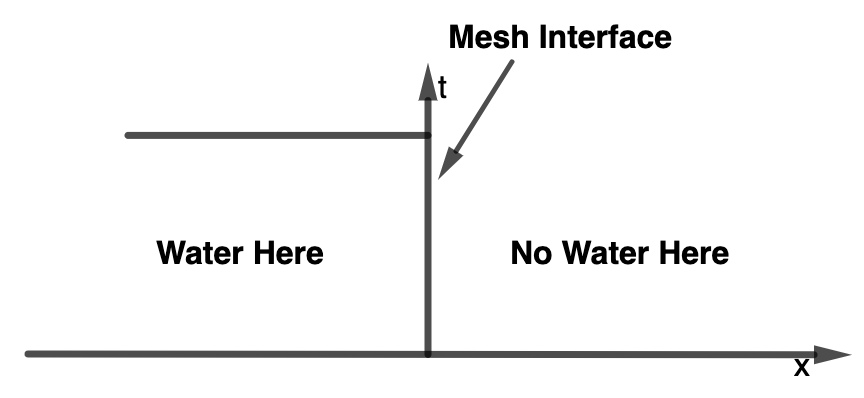
\includegraphics[width=0.5\linewidth]{images/dd1}
		\caption{ The Riemann problem with a dry bed (has no water) in one of the data state. }
		\label{fig:dry-bed}
	\end{figure}
	
	Figure \ref{right}  shows the temporal evolution of the true solution  for the height field for case of a Riemann problem with a right dry state (see Figure \ref{fig:dry-bed}). The solution was obtained using Toro's method implemented in the exact Riemann solver with intial coditions: $h_l  = 1$, $h_r = 0$, and  $u_l = u_r = 0$ described  below.
\begin{figure}[H]
	\subfloat[]{
		\begin{minipage}[c][1\width]{
				0.34\textwidth}
			\centering
			%\caption{}
			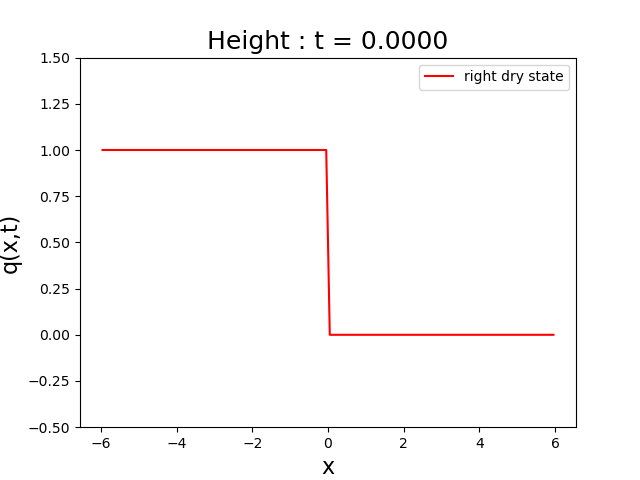
\includegraphics[width=\linewidth, height=5cm]{images/right0}
			\label{fig:right0}
	\end{minipage}}
	\subfloat[]{
		\begin{minipage}[c][1\width]{
				0.34\textwidth}
			\centering
			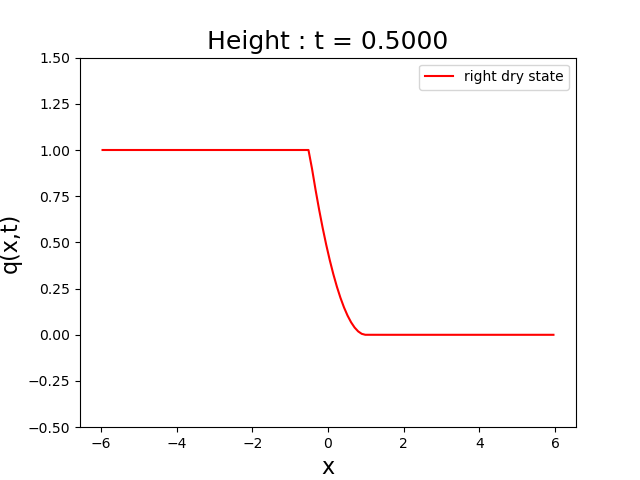
\includegraphics[width=\linewidth, height=5cm]{images/right5}
			\label{fig:right5}
	\end{minipage}}
	\hfill
	\subfloat[]{
		\begin{minipage}[c][1\width]{
				0.34\textwidth}
			\centering
			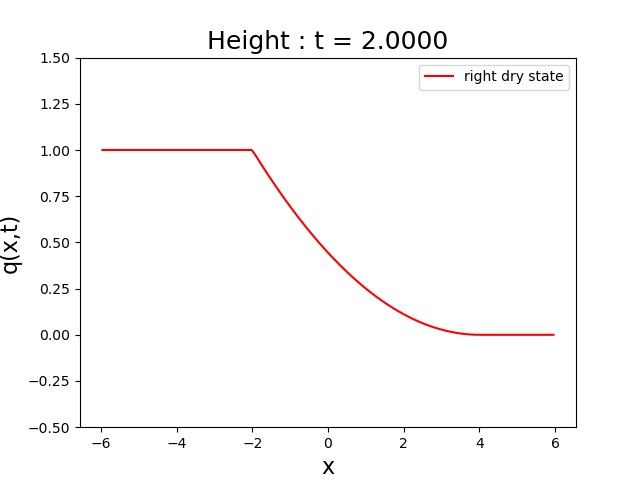
\includegraphics[width=\linewidth,height=5cm]{images/right15}
			\label{fig:right2}
	\end{minipage}}
	\caption{Temporal evolution of the height field solution for the right dry state case  are depicted by (a), (b), and (c) at time steps: $t=0~s$ (initial conditions), $t = 0.3~s$, and $t = 1.0~s$ respectively. }
	\label{right}
\end{figure}

Below, we describe different methods that appear in the literature for handling the wetting and drying problem.

	\subsection{Four elevation modification  method (Liu et al.)}
		\citet{li-ta-wa-ca-ba-ch-li:2021} also used the Godunov-type finite volume methods to process dry and wet/dry front cells to predict flood elevation. This was done by taking four elevation modifications: (1).  Identifying four types of intercell through estimating their properties based on the depth of the flow and surface elevation difference; (2). Updating interface elevation depends on their properties to achieve gravity balance and prevent non-physical flux predictions;  (3).  Calculating dry cell's center elevations by taking the average of the two surrounding intercell elevations; (4). Modifying the first term of the slope limiter based on the elevation difference between intercell elevations dividing two times the mesh size. Furthermore, the first term of the slope limiter function in the dry cell is used to finalize matrix simulation of the entire area and solve the wet/dry problem; this enables SWE application to areas with complex geometry, preventing more elevation modifications.
	
	\subsection{Relaxation method (Pelanti et al.)}

 \citet{pelanti2011riemann} formulated a Rieman solver based on the relaxation approach for both single-phase and double-phase shallow flow equations explaining a mixture of granular material and fluid. This approach is implemented by employing auxiliary variables to replace momenta in the spatial gradients of the original system. The eigenvalues of the relaxation model are determined from the coefficients of the linear equations governing the new auxiliary variables.  The Riemann solution for the height of the flow and relaxation variables are calculated as Roe's Riemann solution; this makes the resulting solver similar to the Roe solver. However, it has the advantage of certain freedom to specify wave speeds by choosing relaxation parameters. This added advantage makes the new solver more robust in handling wet/dry interfaces (\cite{pelanti2008relaxation,pelanti2011riemann}).

	\subsection{Contact discontinuity  Method (Toro)}
	\citet{toro2001shock} solved a Riemann problem with cases in which the dry regions are either present at the initial time or appear as a result of the interaction of two wet bed states. According to his approach, there are three possible cases to consider, as illustrated in fig.~\ref{fig:dry-wet}. Case (a) right dry bed, the solution exhibits a left-going rarefaction ({\em 1-rarefaction}) wave associated with the left eigenvalue $\lambda_1 = u - a$. Case (b) Left dry bed, the solution exhibits right-going rarefaction ({\em 2-rarefaction}) wave associated with the right eigenvalue $\lambda_2 = u + a$. Case (c) dry bed doesn't exit at $t=0$, but is created in the interaction between the two left and right wet bed regions if $S_{*L} \le S_{*R}$ where $a = \sqrt{gh}$.
		\begin{figure}[H]
		\centering
		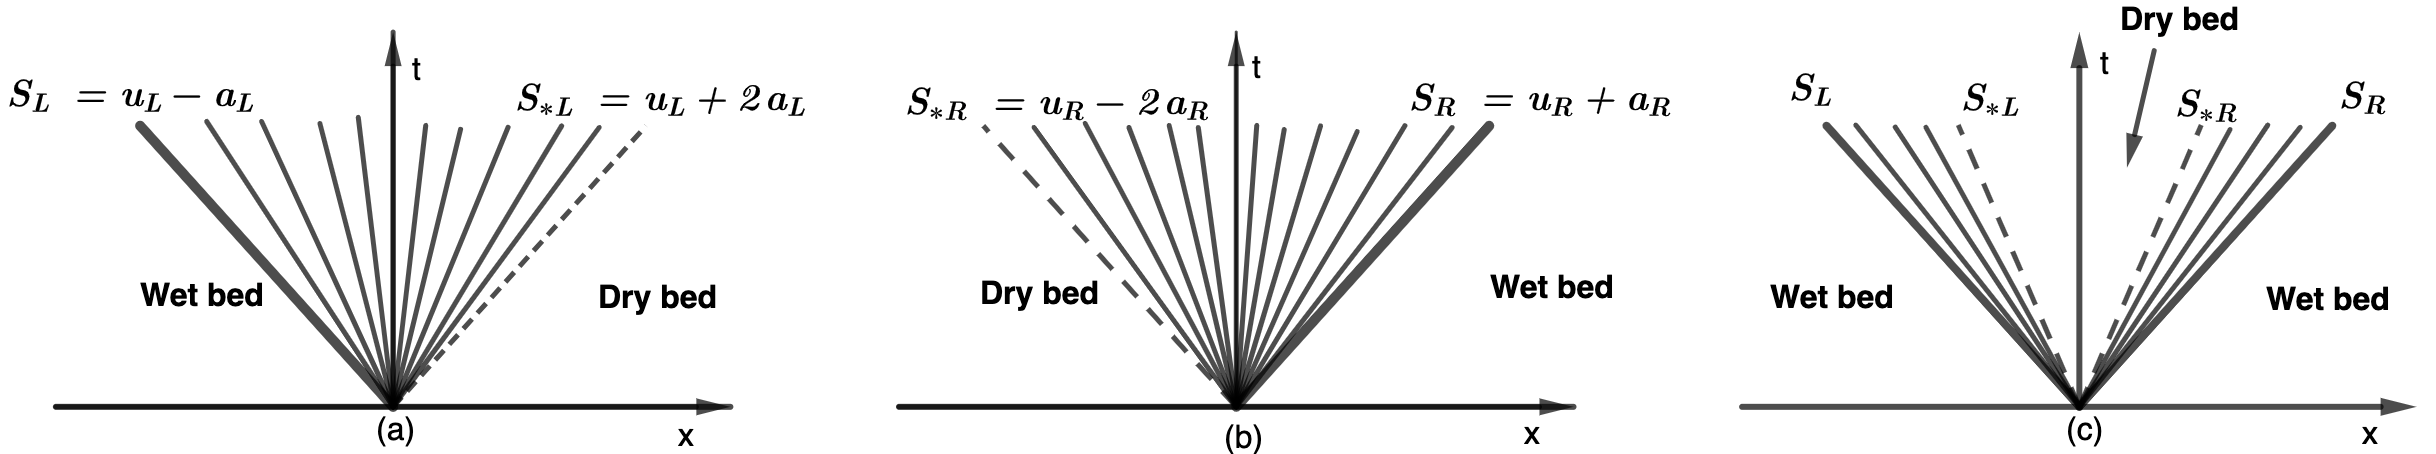
\includegraphics[width=.9\linewidth]{images/dry-wet}
		\caption{The dry state appears in three cases: (a) dry region is on the right, (b) dry region is on the left, and (c) dry region appears in the interaction of two wet bed states. The dashed lines in all figures: (a), (b), and (c) depict the contact discontinuity of speed $S_{*R}$ or $S_{*L}$ that coincides with the tail of the rarefaction in all dry regions. This contact discontinuity is also known as the wet/dry front.}
		\label{fig:dry-wet}
	\end{figure}
	


	\subsection{Galerkin approach (Bunya et al.)}  
		The wetting and drying can also be handled by the linear piecewise  Runge-Kutta discontinuous Galerkin approximation (RKDG)  to SWE solutions;  according to \citet{bu-ku-we-da:2009}, this method is based on the thin water layer approach to optimize both computational cost and accuracy on fixed meshes. The water depth of each dry or partially wet element is tracked and controlled by updating water surface elevations at every end of each Runge-Kutta time step. This maintains the depth positivity of the water column through redistributing mass within each element, which brings about a stable solution over the entire domain for the SWE. In addition, local mass is conserved since the sum of mass inside an element remains constant. The update is independent of the neighboring elements states because it highly depends on the element's velocity and surface elevation. The technique's special treatment of numerical fluxes enables the water mass positivity in each element \cite{bu-ku-we-da:2009,kubatko2007semi}. According to \citet{bokhove2005flooding,bu-ku-we-da:2009}, the locality minimizes the communication between subdomains which improves parallel efficiency. 

	\subsection{Adaptive approach (Popinet)}
\citet{popinet2011quadtree} modeled the 2004 Indian ocean tsunami using adaptive modeling by generalizing the \citet{audusse2004fast} well-balanced and positivity preserving scheme for solving the Saint-Venant equations with wetting and drying to an adaptive quadtree spatial discretization.  Furthermore, an efficient method that dynamically reconstructed multiscale bathymetry depending on vast datasets was discussed.  While Popinet does not provide much detail on how the wetting/drying states are handled, the results in the paper suggest that the method is robust.  Furthermore, the wet/dry state solver is combined with a Boussinesq solver to preserve the robustness of Saint-Venant solver. The adaptive mesh refinement provided higher orders of magnitude gains in memory and speed when the approach was subjected to the dispersive wave propagations that occurred during the Tohoku tsunami.


	\subsection{Augmented Riemann solver (George)}

	\subsubsection{Handling Wetting and drying in the wave propagation algorithm}
	

	In \cite{ge:2008,ge:2011}, a method for handling wetting and drying in the wave propagation algorithm is described.  In this method, it is suggested to replace  equation	\eqref{wpa19} by  \eqref{p5}


	\begin{equation}
		\begin{bmatrix} 
			H_{i} - H_{i-1}\\ 	HU_{i} - HU_{i-1} \\  \varphi(Q_{i}) - \varphi(Q_{i-1}) 
		\end{bmatrix} = \sum_{p=1}^{3} \alpha_{i-\frac{1}{2}}^{p} w_{i-\frac{1}{2}}^{p}
		\label{p5}
	\end{equation}
	where the momentum flux $\varphi(q) = (hu^{2} + \frac{1}{2} gh^{2})$, $Q_{i} = (H_{i},HU_{i})^{T}$ represents the numerical solution of $q = (h,hu)^{T}$ in $C_{i}$, and $w_{i-\frac{1}{2}}^{p} \in \mathbb{R}^{3}$ ,$\forall ~ p \in [1,3] $ with $p$ a set of chosen independent vectors. \\
	
	The decomposition of the solutions $Q_{i} - Q_{i-1} $  and  $f(Q_{i}) - f(Q_{i-1})$ $ \in  \mathbb{R}^{2}$ are represented by the first two and last two components of the three components of the decomposition \eqref{p5} respectively.  Conservation is maintained by modifying fluctuations using the last two of the three components  in equation \eqref{p5} . Then  consider $z_{i-\frac{1}{2}}^{p} \in \mathbb{R}^{2}$ for each $p \in [1,3]$ to be flux waves defined by:
	
	% \donna{why do we need the $\mathbf{I}_{2\times2}$ terms below?}

	\begin{equation}
		z_{i-\frac{1}{2}}^{p} = [\mathbf{0}_{2\times1} \quad \mathbf{I}_{2\times2}] \alpha_{i-\frac{1}{2}}^{p} w_{i-\frac{1}{2}}^{p}
	\end{equation}
	where $\mathbf{0}_{2\times1}$ is a two by one zeros matrix, $\mathbf{I}_{2\times2}$ is a two by two identity. Then updated fluctuations become:
	\begin{eqnarray}
		\mathcal{A^{+}}\Delta Q_{i-\frac{1}{2}}^{n} = \sum_{\{ p:s_{i-\frac{1}{2}}^{p}>0\}}  z_{i-\frac{1}{2}}^{p}
		\label{p7}\\
		\mathcal{A^{-}}\Delta Q_{i+\frac{1}{2}}^{n} = \sum_{\{ p:s_{i+\frac{1}{2}}^{p}<0\}} z_{i+\frac{1}{2}}^{p}
		\label{p8}
	\end{eqnarray}
The decomposition of the four variables: depth, momentum, momentum flux, and bathymetry into four propagating waves give the solver unique features, i.e.,  Riemann problems with a large rarefaction are accurately more approximated, a natural entropy fix for transonic rarefactions,  stationery oceans at a steady-state and discretized smooth, steady states over variable bathymetry are preserved, and shockwave solution is captured due to the solver's equivalency to the Roe solver.
Furthermore, in the absence of the source term, the solver preserves depth negativity and is well balanced in the presence of a source term.  

	\section{ Future research directions}

	
	Several exciting research questions remain unanswered yet, for instance, in the case when eigenvalues of the Jacobian matrix  change sign. Results show that the available approaches, i.e.,  \citet{ba-le-mi-ro:2003} approach, can be applied to problems of that type and obtain high-resolution results; however, the proper treatment of such sonic points is critical. 
	
	Another interesting question is  how to solve the issue of depth negativity in the approximate solver for presence of wet and dry states, when the update term $  \frac{\Delta t}{\Delta x} \left[ \mathcal{F}(Q_{i} , Q_{i+1} ) - \mathcal{F}(Q_{i-1} , Q_{i} ) \right]$ in equation \eqref{cellupdat} becomes larger than $Q_{i}^{n}$  after a few time step. This makes the input height values in the exact solver negative, which breaks the solver, hence we fail to obtain the intermediate state. 

	\begin{itemize}
	%\item Software developments : adaptivity (forestclaw, Basilisk (popinet)), parallelization, GPUs. (\cite{qi-le-mo:2018,po:2015,be-ge-le-ma:2011}) 
	%\item Coupling to other software (an atmospheric code, for example).  Detect tsunami's by looking for signals in the atmosphere.
	\item Modeling questions : dispersive corrections (Serre-Green-Naghdi solver  requiring a linear solver.  Multi-layer SWE also has "dry state" ) (\cite{la-bo:2009,po:2020,po:2015}).
%	\item Implementing SWE on a cubed sphere grid with AMR (\cite{gaudreault2021high})
	\end{itemize}


Tsunamis can also be detected in real-time through observation of signals in the atmosphere. The occurrence of earthquakes triggers tiny atmospheric waves that propagate through the earth's surface to the ionosphere. These tiny waves cause detectable changes to the density of electrons in the ionosphere, which can be measured and recorded by the global navigation satellite systems (GNSS). 
Once a tsunami forms and moves across the ocean, it generates waves with crests and troughs, which compress and expand the air above them. This creates gravity waves (motions in the atmosphere) which are amplified as they travel upward into the atmosphere.  GNSS satellites detect these waves once they reach the ionosphere.  Detecting both the gravity waves and electron density variations in the ionosphere by the GNSS can help us detect both the location of the earthquake and the movements of the tsunami in real-time. 
Also, existing software for predicting tsunamis can be incorporated with other atmospheric models to improve forecasts. For instance, Variometric Approach for Real-time Ionosphere Observation (VARION)  is coupled with tsunami detection systems based on data from various sources: seismometers, ocean bottom pressure sensors, buoys, and GNSS receivers (\cite{savastano2017real}). Once an earth quate is detected in a region, VARION starts to process real-time measurements of the distribution of electrons from several ground stations near the earthquake's epicenter while searching for changes correlating to the expected formation of a tsunami.


	
	Apart from using single programming SWE models described above in this paper, tsunami simulations can also be handled by parallel programming models, which also use finite volume solvers.  The computational domain may be obtained using patches of cartesian grids connected via ghost layers. Then the FVM can be restricted to piecewise constant approximation in each grid cell. The fluxes between cells may be computed using the Lax-Friedrichs,f-wave, Argumented Riemann solver, or any hybrid solver. We can then use GPUS (executing CUDA kernels), MPI (data exchange), OpenMP(loop parallelism), etc., to study parallelization of this model through testing and comparing of weak and strong scaling plots (\cite{qi-le-mo:2018}).  We also plan to test SWE on software with adaptivity: forestclaw (\cite{be-ge-le-ma:2011}) and  Basilisk (\cite{po:2015})

	We are also interested in implementing SWE on a cubed sphere grid with adaptive mesh refinement (AMR).  According to \citet{mccorquodale2015adaptive}, this can be modeled with multiblock grids by combining a Runge-Kutte time discretization with a fourth-order accurate spatial discretization that includes adaptive mesh refinement and refinement in time.  We think this can also be obtained by subjecting the SWE to locally refined uniform grid finite volume discretization on the sphere's surface. We also anticipate using immersed boundary methods (\cite{lundquist2010immersed}, terrain-following coordinates, and coupling climate cloud microphysics to apply AMR to very high-resolution simulations.
	
	
	
	
	%\nocite{*}
	
	\bibliographystyle{abbrvnat}
	% \bibliographystyle{plain}
	\bibliography{geoclaw,literature}
	
\end{document}

